\documentclass[10pt,letterpaper]{article}

\usepackage[margin=0.75in]{geometry}
\usepackage{tikz}
\usepackage{amsfonts}
\usepackage{listings}
\graphicspath{ {images/} }

\begin{document}

  \title{CS 476, Assignment 1}
  \author{Cody Malick\\
  \texttt{malickc@oregonstate.edu}}
  \date{\today}
  \maketitle

\section{}
\subsection*{Graph}
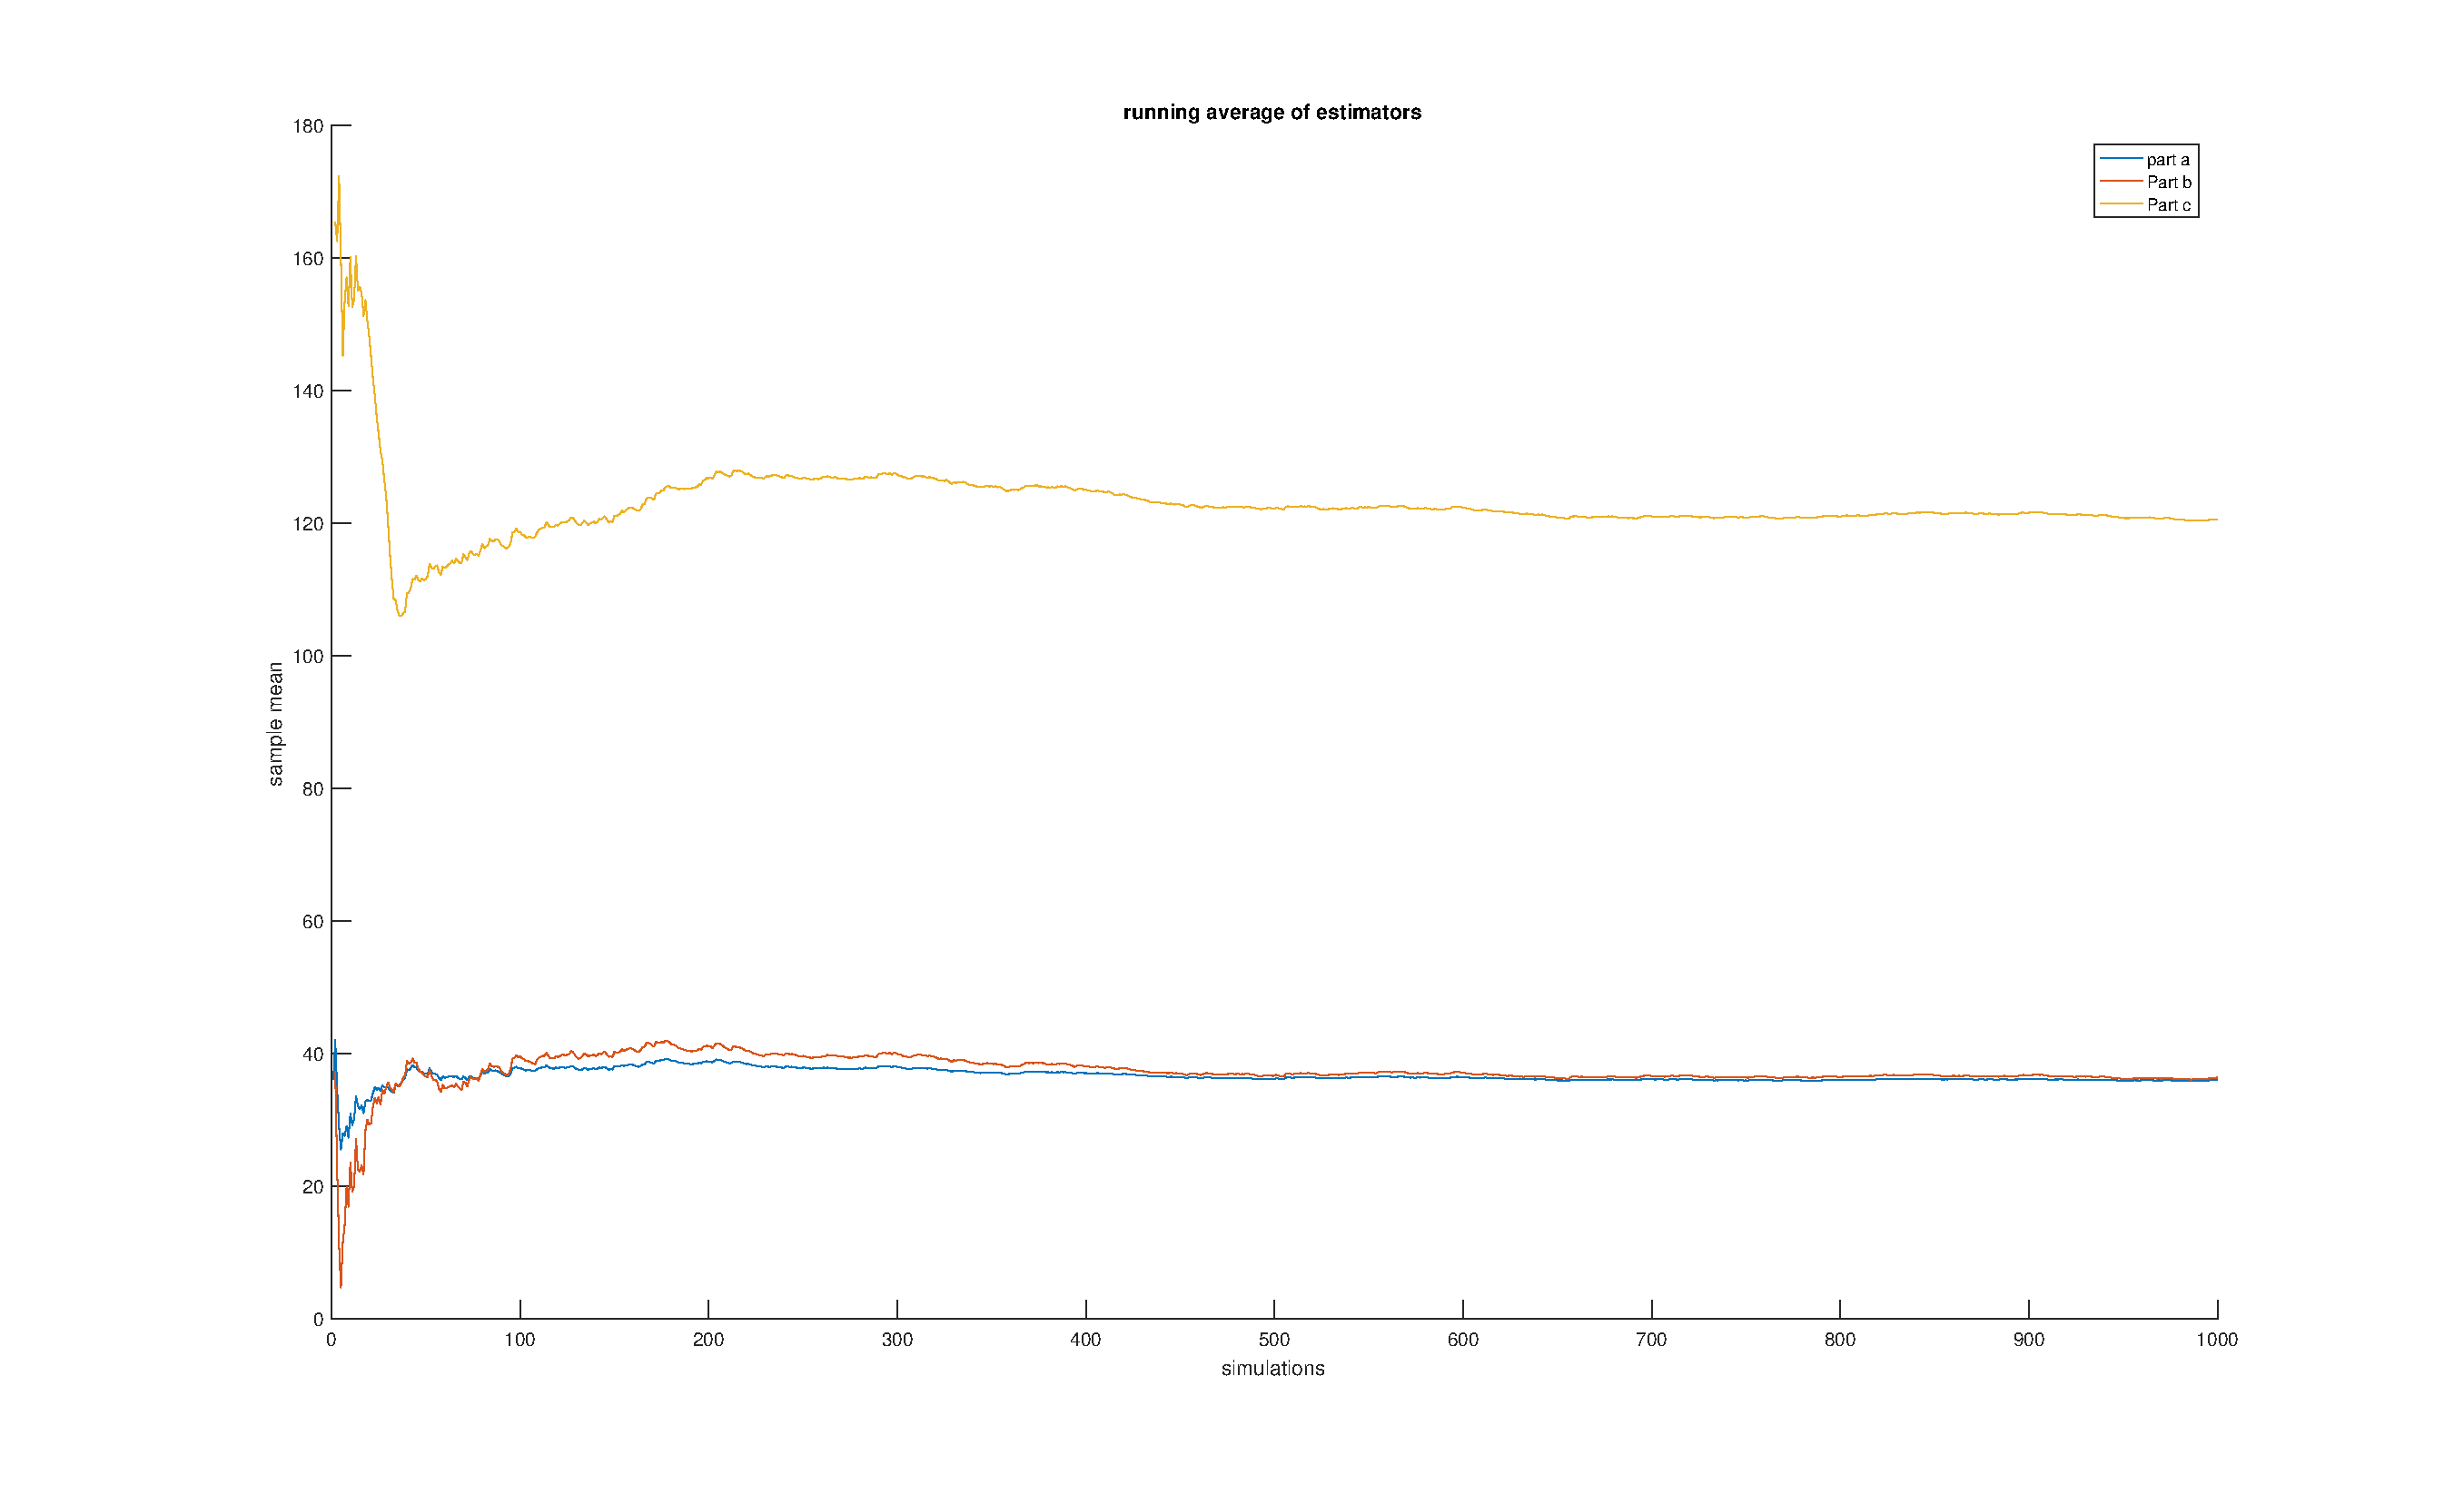
\includegraphics{assignment1.eps}
	\subsection*{a}
	The simple estimator approached the value of theta in fairly short order,
	though not as quickly as the first conditioning variable.
	\subsection*{b}
	Looks like it approaches the true value of theta faster than the 
	naive approach.
	\subsection*{c}
	I wasn't able to get this one working completely. I was unsure as to
	what it was in my code that was offsetting it by so much.
	\subsection*{d}
	Unfortunately, I was unable to get started on this one.

\section{}
	
\end{document}
